\clearpage
\section{Design Verification Process}\label{section:prototype_validation}

The development of the AFE hardware was separated from the software controlling it, in practice meaning that the verification of the hardware design by measuring its performance in different situations was the software team's (for the most part, the author's) responsibility, although the hardware team did provide some support in interpreting the results.

The verification was begun by analyzing the very first prototypes of the AFE, put together on the same board with a microcontroller and a power supply, and continued with the second round of prototypes where the microcontroller and the AFE were more tightly bound and shielded. The aim of the verification process was to determine the system's operating limits and properties and to analyze the noise behavior of individual subsystems and the system as a whole with different settings.

The verification process was made difficult by the fact that the AFE has such a wide range of options -- to find the optimal set of timings and other control values was no easy task and took a lot of effort and analyzing. In the following chapters the methods applied to the task are explained.

\subsection{Regression Analysis}

Regression analysis is a collection of statistical methods for modeling and analyzing a system, the focus being on identifying system variables and/or parameters and their relationships \cite{Kleinbaum2007}. In this particular case regression analysis can be used to estimate the performance of the different subsystems by carefully selecting the dependent variable and varying one as carefully picked independent variable (i.e. a system parameter) at a time.

\subsection{Methodology Used}

The fundamental issue with analyzing the performance of the chip is that the analyzing equipment and wiring should be much less noisy than the system to be analyzed in order to get any reliable and quantifiable results. As the noise levels in question are extremely small it posed some restrictions on how the validation could be done -- therefore it was decided to design a set of tests that could be done using the system itself and that would provide data about both the system as a whole and about individual subsystems.

The tests were made to be a set of measurement series, in each of which only one measurement parameter was changed. By combining data from these measurements it was possible to determine how each of the subsystems performed with different settings using regression analysis and to find the optimal operating modes for different use cases using only the AFE's transmitter as the stimulus and the AFE's receiver as the data collector.

The key to the making up of the tests is to know the system completely. Many of the configurable parameters in the measurement are intertwined, rendering isolated changes in one of them pointless unless one knows how it really will affect the system. An example of such interconnections is LED pulse length: not only does it affect the required sampling time and resulting sampling noise, but also the low-pass filter composed of the RC feedback circuit must be tuned so that the corner frequency is sufficient for passing the pulse without too much distortion. Therefore the measurement parameters weren't always atomic values but combinations of them previously identified as isolated, correlated sets of values. In short, a lot of effort was put into analyzing the dependencies between the system variables and isolating independent combined parameters.

\subsection{Embedded Software Design}

The software used within the microcontroller was designed and implemented so that it would both support the verification process and eventually end up as the final product software. This required a kind of agile development method based on Scrum \cite{Schwaber2009} where each iteration produced a usable product with more functional features than the previous one, the order of development highly guided by the progress of the verification process. The verification required a number of features not needed in the final product which meant that they had to be well isolated from the core program, dependencies being strictly unidirectional. The embedded software was written in Embedded C++, using IAR's compiler and linker \cite{IAR}.

In the evaluation phase the software had two key features: as all control and analysis was done externally it had to be able to fetch the measurements from the ADC and send them through a serial link to a PC and it had to be able to receive commands from said link and set AFE control values accordingly. This meant that the very first pieces of software implemented were the drivers and higher-level manager classes of both the SPI interface for the ADC and the UART interface for PC communication, naturally using the communication protocol selected for the final product. Gradually the number of features was increased, starting from calculating some combinations of control values based on input and moving on to handling the diagnostics and automatically setting all the control values based on measured signal level and desired power mode. The development paradigm supported simultaneous verification and software development very well and proved to be successful throughout the project.

\begin{figure}[htcb]
\begin{center}
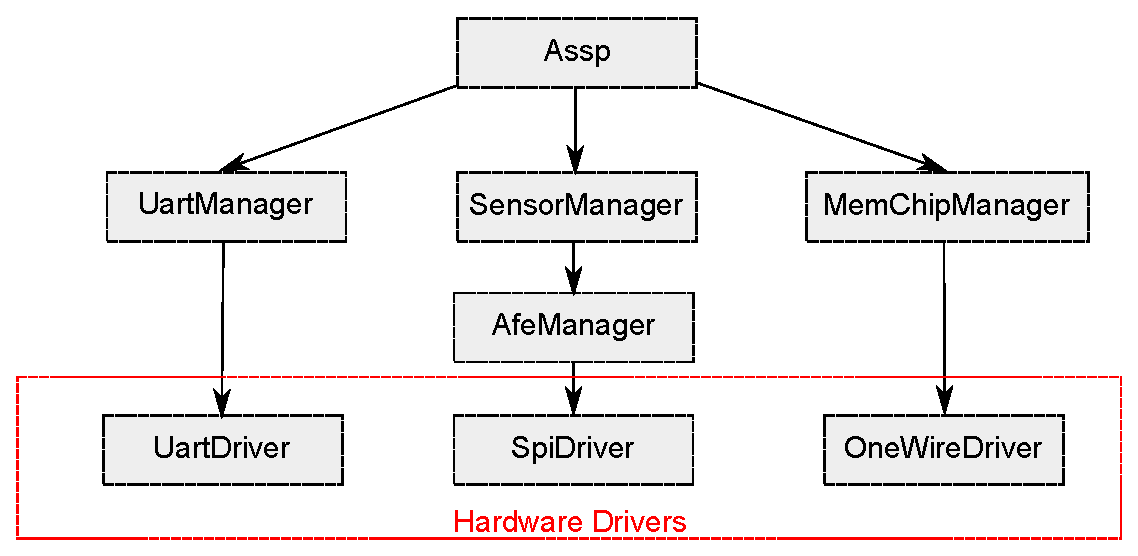
\includegraphics[scale=0.75]{kuvat/assp_class_diagram.eps}
\caption{The structure of the embedded software of the MSP430 microcontroller.}
\label{fig:assp_class_diagram}
\end{center}
\end{figure}

Figure \ref{fig:assp_class_diagram} shows the class structure of the software. It can be seen that the communication interfaces are separated from the rest of the code, providing a platform that doesn't take any position on its usage. All the received commands are handled in the main program -- in fact, all the validation-only code is confined in the 'Assp' class. Also, the communication drivers tightly bound to hardware are separated from the manager classes to provide sufficient abstraction and thus more portable code.

The program is based on interrupts raising flags that trigger actions in the main program. For example, the end of an A/D conversion is indicated by raising a flag in an interrupt service routine. The main program detects it and executes the measurement fetching subroutine when it has finished any ongoing task. This approach makes sure that the response time is always rather fast but also that no ongoing task gets blocked by overly processor-intensive interrupt handlers. On the other hand, using hardware-dependent interrupts makes automated testing of the code difficult and impractical; because of this several manually-run tests were written to ensure code integrity.

\subsection{PC Software Design}

The analysis software, shown in figure \ref{fig:HkiAsspADE}, was built on top of Matlab using its proprietary scripting language and user interface designer. The goal of the software was to provide a tool for setting the AFE parameters and evaluating the result online, and also for capturing data for offline analysis. The user interface shows the output and its power spectrum as graphs, the AFE's control values as a list and provides an interface for changing any or all of them. 

\begin{figure}[htcb]
\begin{center}
  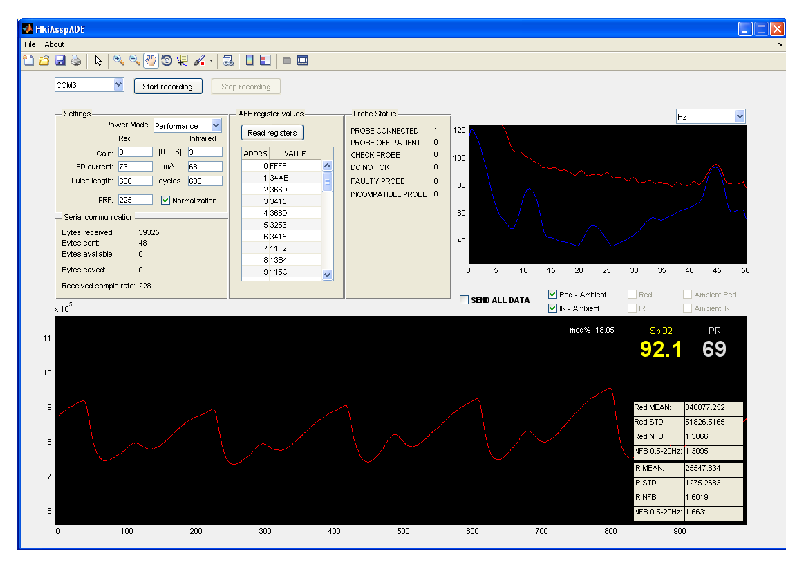
\includegraphics{kuvat/HkiAsspAde.eps}
  \caption{The PC software used to remotely control the measurement system with features for visualizing and processing both the incoming samples and the system's internal state.}
  \label{fig:HkiAsspADE}
\end{center}
\end{figure}

\subsection{Critical Tests and Derived Parameters}

After being established that all the features of the AFE work as intended, the most important property of the system to evaluate is its noise performance as indicated in chapter \ref{section:noise_characterization}, and in the case of not immediately reaching the target, identifying the dominant noise source. Methods for this include plotting measured system noise as functions of receiver gain, transmitter current, pulse length, pulse repetition frequency, and other variables. From the results it's possible to deduce with reasonable accuracy the amount of noise each subsystem contributes to the final figure by fitting a theoretical model on the measurements.

The components producing noise in the signal chain can be listed as follows:
\begin{itemize}
	\item Transmitter noise (current variability from one pulse to another, timing jitter)
	\item Photodiode noise (shot noise) and settling time
	\item Noise induced into the photodiode cable leads from the environment and LED leads
	\item Thermal noise in the conductive path
	\item Receiver op-amp noise
	\item Sampling noise
	\item A/D conversion noise.
\end{itemize}

Transmitter noise can be identified to some extent by measuring the receiver noise floor without the transmitter and then measuring with the same settings, only this time with transmitter on. Similarly, the effect of the photodiode and the cable can be identified by replacing the sensor with a dummy block. The tests performed are explained more thoroughly in the next chapter but the key to the analysis is to identify the alterable system parameters that affect only the performance of a single subsystem.

\subsubsection{Distinguishing Amplifier Noise From Sampling and Conversion Noise}

With zero input (photodiode pins connected through a big resistor), it is assumed that all noise in the receiver output is due to suboptimalities in three distinct subsystems: the cross-impedance amplifier, the sampling unit and the conversion unit. Since all noise produced before the amplifier stage including the operational amplifier's noise itself gets amplified, with zero signal the amplifier noise is assumed to have a somewhat linear relationship to the gain used. Everything after the amplifier on the other hand should be rather constant with respect to gain, meaning that measuring system noise as a function of gain should result in an estimate of the magnitudes of the effective noises of the individual subsystems.

As said, the sampling and conversion noises are virtually unaffected by receiver gain. The key parameter determining sampling noise is sampling time, the relationship being inverse like the relationship between conversion noise and conversion time as well. Additionally, all the noise components are assumed to be white and uncorrelated, meaning that their magnitudes add into each other in a root-mean-square manner. These assumptions give us a rudimentary model of the noise system of the receiver:

\begin{equation}
  \begin{array}{ccl}
	\sigma_{receiver} &=& \sqrt{ (a \cdot R_f)^2 + (\frac{b}{\tau_s})^2 + (\frac{c}{\tau_c})^2} \\
	\sigma_{receiver}(R_f) &=& \sqrt{ (a \cdot R_f)^2 + \sigma_{sc}^2} 
	\end{array}
	\label{eq:receiver_noise_model}
\end{equation}

If plotted as a function of $R_f$ the result could be something like in figure \ref{fig:receiver_noise_model} -- The part of the noise not related to $R_f$ can be clearly identified from the point $R_f = 0$, making the estimation of the parameter $a$ an easy task. Similar plot can be drawn for the noise as a function of conversion time, but not for sampling time -- sampling time also defines the optimal corner frequency of the amplifier feedback low-pass filter which makes the two connected.

\begin{figure}[htcb]
\centergraphics{kuvat/receiver_noise_model.eps}
\caption{Estimated system noise according to the model in equation (\ref{eq:receiver_noise_model}) plotted as a function of $R_f$.}
\label{fig:receiver_noise_model}
\end{figure}

\subsubsection{Distinguishing Transmitter Noise From Receiver Noise}

In previously examining the receiver only zero input signal was used. That might impose a problem when trying to assess transmitter noise by directly measuring the noise of the system when used as indicated in figure \ref{fig:validation_system_setup} since the receiver might not perform identically with a signal that has a non-zero DC level. Therefore a measurement circuit was devised that would allow measuring the transmitter's noise behavior in DC mode as a function of LED current, illustrated in figure \ref{fig:tx_dc_test_setup}. That is not enough, though, as the transmitter's performance must also be examined in pulsating mode.

\begin{figure}[htcb]
\centergraphics{kuvat/validation_system_setup.eps}
\caption{The setup of the validation. A standard sensor with a light attenuation block is used as the transmitter-receiver coupling device. As the attenuation block is static the output signal should be a DC one, which allows using the output's standard deviation as the primary measurement quality indicator.}
\label{fig:validation_system_setup}
\end{figure}

\subsubsection{Receiver Noise with a Dynamic Signal}

The big problem in identifying the receiver performance in normal operating conditions is that it's very difficult to produce a pulsed reference input signal small and noiseless enough so that it could be used to measure the receiver's dynamic behavior. As the DC measurements defined earlier don't tell much of the receiver's performance in normal operation, this is both interesting and crucial in assessing the performance of both the receiver and the transmitter: If such a signal is available it can be used to determine the receiver's noise which in turn can be used to calculate the noise component caused by the transmitter in normal operation.

The main challenge with the reference signal is that its amplitude must be very small to avoid saturating the receiver; the maximum current should be in the range of 0.5-25 $\mu$A depending on the receiver gain setting which is a lot to ask from most signal generators, especially as its noise level should be well below the receiver's. Also, to simulate a typical pulse oximetry signal the reference signal should be pulsed and synchronized to the measurement cycle so that the top of the square wave coincides with signal sampling.

Perhaps the most useful input signal for characterizing the receiver only would be a pulsed one which is amplitude modulated with an approximately 0.5-5 Hz (30-300 bpm, normal cardiac range) pure sinusoidal signal. It could be used to measure the receiver's critical characteristics such as noise, distortion, harmonic noise, linearity and phase response by comparing the measured signal to the ideal one.

\subsubsection{Transmitter Noise in Normal Operation}

The specifications of the transmitter claim that its signal-to-noise ratio is constant throughout the dynamic range. As the noise caused by the receiver is measured in the previous test, it is fairly simple to estimate the effect of the transmitter as a function of LED current with the following equation:

\begin{equation}
  \sigma = \sqrt{(k \cdot I_{LED})^2 + \sigma_{Rx}^2} .
  \label{eq:sigma_Tx}
\end{equation}

Again, it is assumed that the different noise components are white and uncorrelated -- in actual operation this might not be the case if e.g. noise originating from the power supply is summed up into both the transmitted and the received signal or if there's significant crosstalk between the transmitter and the receiver. For the purposes of testing only the AFE the assumption is enough, though.